\chapter{Introduction: The Vulnerability Prioritization Crisis}
\label{chap:introduction}

\section{The Threat Landscape and Alert Fatigue}
In contemporary enterprise architectures, vulnerability management programs are confronted with an unprecedented volume of Common Vulnerabilities and Exposures (CVEs). Organizations routinely receive tens of thousands of automated scanner findings per month. In practice, operational security teams (SecOps) cannot patch all reported defects within typical service level agreements (SLAs).

The primary challenge lies in \textbf{alert inflation}: conventional scanners evaluate vulnerability severity based heavily on source CVSS assessments published by vulnerability authorities and commonly indexed by services such as the National Vulnerability Database (NVD)~\cite{first_cvss_v4}. A remote code execution (RCE) defect assigned a CVSS Base score of 9.8 is treated as an existential emergency regardless of whether the affected host is an edge-facing payment gateway or an isolated development sandbox accessible only over a local loopback interface.

\begin{figure}[htbp]
    \centering
    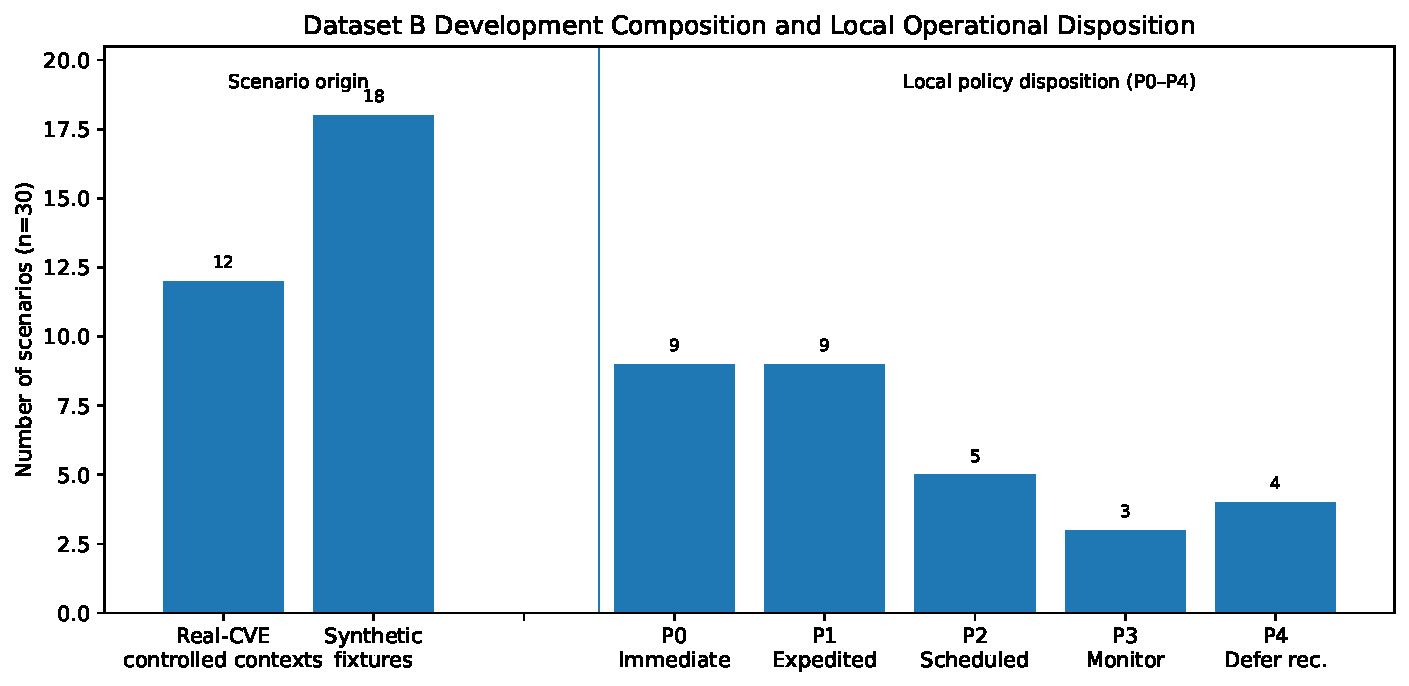
\includegraphics[width=0.96\linewidth]{figures/fig1_dataset_composition.pdf}
    \caption{Dataset B development composition shown without conflating CVSS severity with local policy. The left group identifies scenario origin (12 real-CVE records embedded in controlled contexts and 18 synthetic fixtures); the right group shows legacy local P0--P4 development-policy dispositions. The chart is descriptive development evidence only; it is not an accuracy, false-positive, or held-out validation result.}
    \label{fig:severity_redistribution}
\end{figure}

\section{The Dilemma of Intrinsic Severity vs. Operational Context}
The fundamental mathematical and semantic boundary of vulnerability management is delineated by two concepts:
\begin{enumerate}
    \item \textbf{Base Severity ($S_{\text{base}}$):} Represents vulnerability characteristics that are intended to remain independent of a specific organization's environment. Local compensating controls and business requirements are deliberately outside the Base metric group.
    \item \textbf{Contextual Environmental Severity ($S_{\text{env}}$):} Represents a CVSS Environmental result after organization-specific modified metrics and security requirements have been documented. It is a contextual severity score, not a complete probabilistic risk estimate.
\end{enumerate}

FIRST CVSS v4.0 defines Environmental metrics so that local conditions can be represented explicitly. Applying those metrics at scale may require analysts to reconcile vulnerability records with topology, reachability, asset requirements, and compensating controls. Prior empirical work shows that such contextual assessment becomes error-prone in complex network scenarios~\cite{santos2017estimating}. This work therefore studies whether verified operational evidence can support a more reproducible and auditable recommendation process.

\section{The HelpUS Solution and Research Objectives}
This work introduces the \textbf{HelpUS CVSS Framework}, an evidence-grounded decision architecture that derives \emph{candidate} CVSS v4.0 Environmental metrics from verified operational evidence and then delegates numerical scoring to a specification-conformant CVSS v4.0 calculator. 

Our core contributions are structured as follows:
\begin{itemize}
    \item \textbf{Tripartite Evidence Contract:} Preservation of the source CVSS assessment vector and nomenclature alongside the contextual result and its provenance, supporting auditability without overwriting the original assessment.
    \item \textbf{Deterministic AI Watcher:} An evidence-constrained inference layer that recommends candidate Environmental metrics and abstains when the evidence is incomplete or contradictory.
    \item \textbf{Inverse Environmental Optimization (What-If Solver):} A constrained combinatorial solver that deduces the minimal set of compensating controls required to meet organizational risk thresholds.
    \item \textbf{Policy-as-Code Virtual Patching:} Synthesis of candidate Linux \texttt{iptables}, cloud security-group, and WAF controls that require validation and Human-in-the-Loop approval before production deployment.
    \item \textbf{Reachability-Adjusted EPSS Heuristic:} A clearly labeled heuristic for combining global exploit-likelihood information with local reachability evidence; it is not presented as a calibrated posterior probability.
    \item \textbf{Human-in-the-Loop (HITL) Governance \& SLA Clock:} An auditable 4-step review workflow designed to support organizational governance and alignment with relevant NIST/ISO practices, with tamper-evident provenance and configurable SLA policy.
    \item \textbf{Empirical Scientific Benchmark:} A 30-scenario preliminary benchmark reporting priority redistribution, traceability, abstention behavior, and engine-level latency; accuracy claims require an independently adjudicated expert reference set.
\end{itemize}
